\documentclass[journal]{../../IEEEtran/IEEEtran}

\usepackage[activeacute, spanish]{babel} % p/idioma espaniol
\usepackage[utf8]{inputenc}
\usepackage[T1]{fontenc}
\usepackage{cite}


% *** GRAPHICS RELATED PACKAGES ***
%
\ifCLASSINFOpdf
\usepackage[pdftex]{graphicx}
\usepackage{float}
  % declare the path(s) where your graphic files are
  % \graphicspath{{../pdf/}{../jpeg/}}
  % and their extensions so you won't have to specify these with
  % every instance of \includegraphics
  % \DeclareGraphicsExtensions{.pdf,.jpeg,.png}
\else
  % or other class option (dvipsone, dvipdf, if not using dvips). graphicx
  % will default to the driver specified in the system graphics.cfg if no
  % driver is specified.
  % \usepackage[dvips]{graphicx}
  % declare the path(s) where your graphic files are
  % \graphicspath{{../eps/}}
  % and their extensions so you won't have to specify these with
  % every instance of \includegraphics
  % \DeclareGraphicsExtensions{.eps}
\fi


% *** MATH PACKAGES ***
%
%\usepackage{amsmath}
% A popular package from the American Mathematical Society that provides
% many useful and powerful commands for dealing with mathematics.
%
% Note that the amsmath package sets \interdisplaylinepenalty to 10000
% thus preventing page breaks from occurring within multiline equations. Use:
%\interdisplaylinepenalty=2500
% after loading amsmath to restore such page breaks as IEEEtran.cls normally
% does. amsmath.sty is already installed on most LaTeX systems. The latest
% version and documentation can be obtained at:
% http://www.ctan.org/pkg/amsmath


% *** SPECIALIZED LIST PACKAGES ***
%
%\usepackage{algorithmic}
% algorithmic.sty was written by Peter Williams and Rogerio Brito.
% This package provides an algorithmic environment fo describing algorithms.
% You can use the algorithmic environment in-text or within a figure
% environment to provide for a floating algorithm. Do NOT use the algorithm
% floating environment provided by algorithm.sty (by the same authors) or
% algorithm2e.sty (by Christophe Fiorio) as the IEEE does not use dedicated
% algorithm float types and packages that provide these will not provide
% correct IEEE style captions. The latest version and documentation of
% algorithmic.sty can be obtained at:
% http://www.ctan.org/pkg/algorithms
% Also of interest may be the (relatively newer and more customizable)
% algorithmicx.sty package by Szasz Janos:
% http://www.ctan.org/pkg/algorithmicx



% *** PDF, URL AND HYPERLINK PACKAGES ***
%
\usepackage{url}
% url.sty was written by Donald Arseneau. It provides better support for
% handling and breaking URLs. url.sty is already installed on most LaTeX
% systems. The latest version and documentation can be obtained at:
% http://www.ctan.org/pkg/url
% Basically, \url{my_url_here}.




% *** Do not adjust lengths that control margins, column widths, etc. ***
% *** Do not use packages that alter fonts (such as pslatex).         ***
% There should be no need to do such things with IEEEtran.cls V1.6 and later.


% correct bad hyphenation here
\hyphenation{op-tical net-works semi-conduc-tor}


\begin{document}
\title{Calculadora graficadora.\\Manual de Usuario.}


\author { W.~E.~S.~Tubín \thanks{W.~E.~S.~Tubín actualmente
    estudia en Ingeniería en Ciencias y Sistemas de la Universidad de
    San Carlos de Guatemala. } }


% The paper headers
\markboth{Universidad de San Carlos, Mayo~2018. \LaTeX\  }%
{Shell \MakeLowercase{\textit{et al.}}: Bare Demo of IEEEtran.cls for IEEE Journals}

\maketitle

% As a general rule, do not put math, special symbols or citations
% in the abstract or keywords.
\begin{abstract}
  Este documento muestra el uso de la aplicación, desarrollada en
  asembler usando NASM y emulado desde DOSBox.
\end{abstract}


\begin{IEEEkeywords}
Consola, Ensamblador, Lenguaje.
\end{IEEEkeywords}



% For peer review papers, you can put extra information on the cover
% page as needed:
% \ifCLASSOPTIONpeerreview
% \begin{center} \bfseries EDICS Category: 3-BBND \end{center}
% \fi
%
% For peerreview papers, this IEEEtran command inserts a page break and
% creates the second title. It will be ignored for other modes.
% \IEEEpeerreviewmaketitle



\section{Introducción}
% The very first letter is a 2 line initial drop letter followed
% by the rest of the first word in caps.
% 
% form to use if the first word consists of a single letter:
% \IEEEPARstart{A}{demo} file is ....
% 
% form to use if you need the single drop letter followed by
% normal text (unknown if ever used by the IEEE):
% \IEEEPARstart{A}{}demo file is ....
% 
% Some journals put the first two words in caps:
% \IEEEPARstart{T}{his demo} file is ....
% 
% Here we have the typical use of a "T" for an initial drop letter
% and "HIS" in caps to complete the first word.
\IEEEPARstart{E}{ste} documento da un panorama de como usar la
calculadora graficadora. Es emulada por Dosbox utilizando el
ensamblador NASM. Se utilizaron operaciones básicas a nivel
ensablador, interrupciones, uso de memoria en programas informáticos,
operaciones aritméticas básicas, con signo, a bajo nivel.


\section{Derivar función}

* Presionar 1 en el menú principal\\

* Ingresar ecuación\\
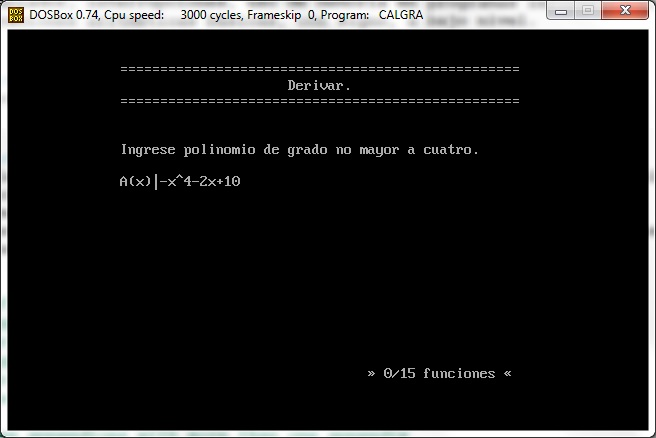
\includegraphics[scale=0.42]{img/11.jpg}

* Presionar la tecla Enter\\

* Muestra mensaje si la cadena es correcta y deriva\\
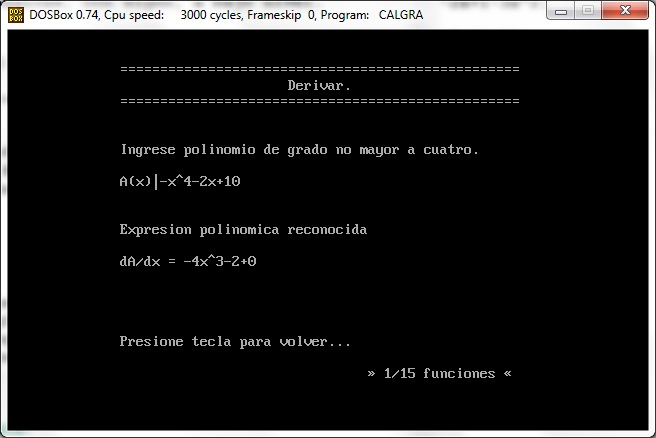
\includegraphics[scale=0.42]{img/12.jpg}

\section{Integrar función}

* Presionar 2 en el menú principal\\

* Ingresar ecuación\\
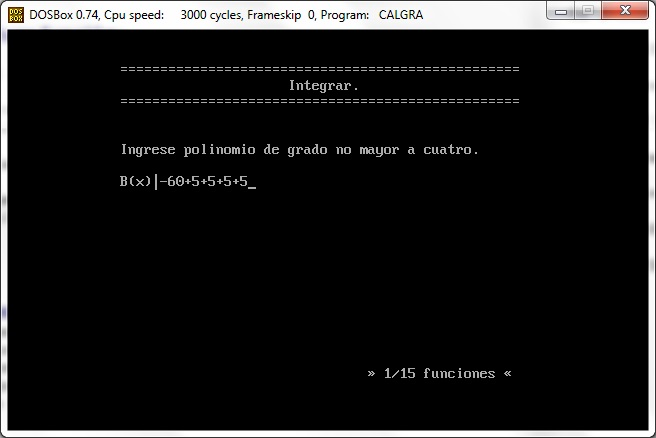
\includegraphics[scale=0.42]{img/21.jpg}

* Presionar la tecla Enter\\

* Muestra mensaje si la cadena es correcta e integra\\
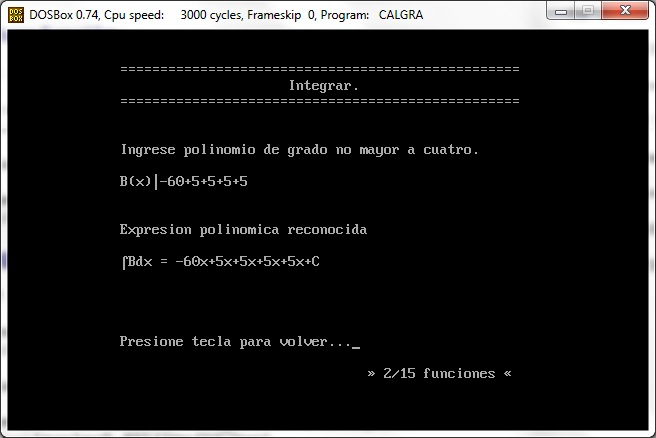
\includegraphics[scale=0.42]{img/22.jpg}

\section{Ingresar funciones}

* Presionar 3 en el menú principal\\

* Escribir la ruta del archivo a cargar\\

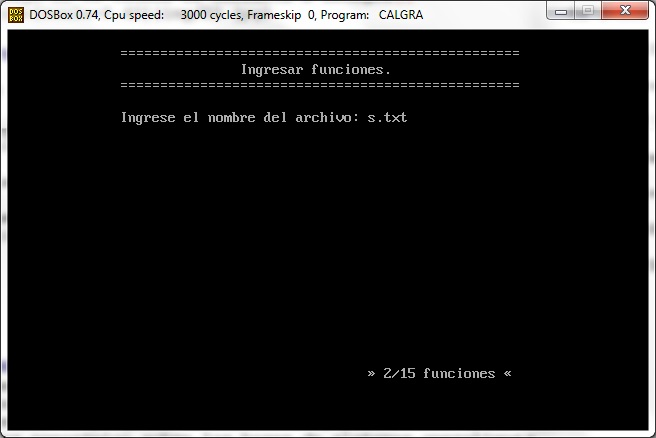
\includegraphics[scale=0.42]{img/31.jpg}

* Presionar la tecla Enter\\

* Escojer la operacion. Presionar 1 si se quiere derivar e integrar
los polinomios que contiene el archivo cargado. Presionar 2 si se
quiere resolver. Al lado derecho del archivo cargado habrá una letra A
si actualmente el archivo esta abierto. Una C si el archivo esta
cerrado y una N si se dejo de operar con el archivo y por algun error
no se cerro el archivo.\\

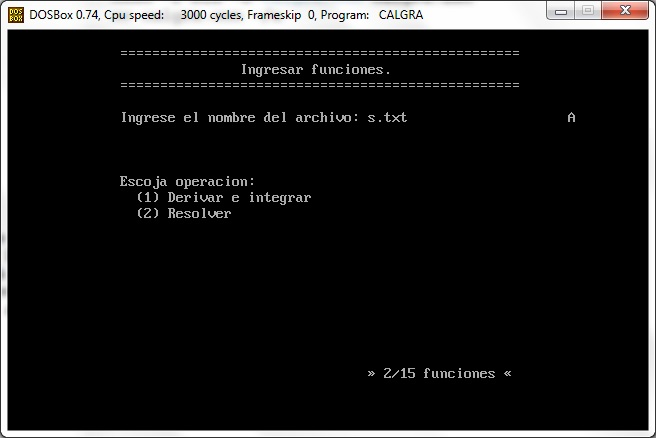
\includegraphics[scale=0.42]{img/32.jpg}

* Se muestra el pantallazo para la opcion 2. Automaticamente calcula
las soluciones enteras. Luego pregunta si desea seguir leyendo el
archivo. Presione la tecla ''s'' para continuar y ''n'' para cerrar el
archivo y regresar al menú principal.\\

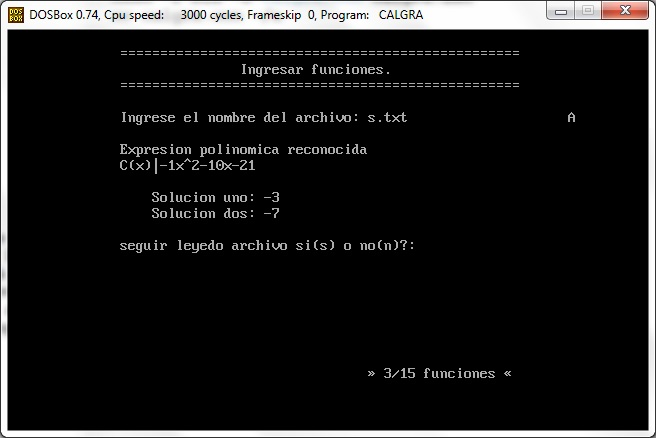
\includegraphics[scale=0.42]{img/33.jpg}

* Además el contador de funciones aumenta si es reconocida una
expresión. Si no es reconocida muestra el mensaje de error la fila,
columna y caracter del error ocurrido. A continuación el pantallazo si
se escoje ''n'':\\

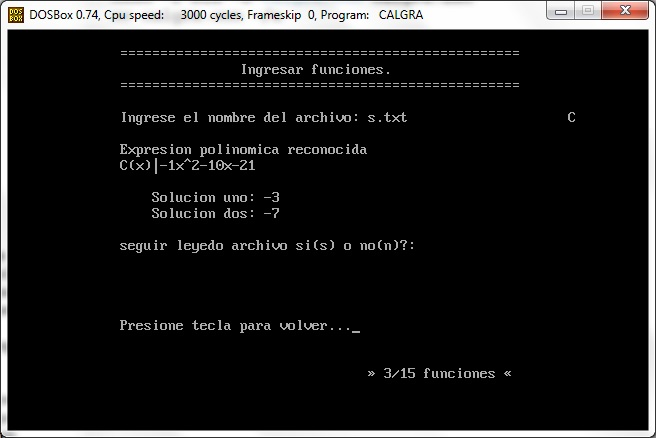
\includegraphics[scale=0.42]{img/34.jpg}



\section{Imprimir funciones ingresadas}

* Presionar 4 en el menú principal\\

* Se muestran las funciones guardados en memoria\\

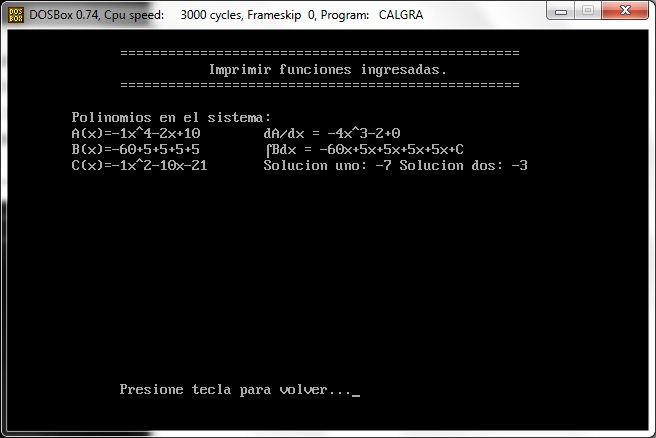
\includegraphics[scale=0.42]{img/41.jpg}

* Presionar cualquier tecla para regresar al menú principal\\


\section{Graficar}

* Presionar 5 en el menú principal\\

* Ingrese un rango de graficación del eje x, los valores pueden ser de
-100 a 100 siempre teniendo en cuenta que el limite inferior debe ser
menor que el superior\\

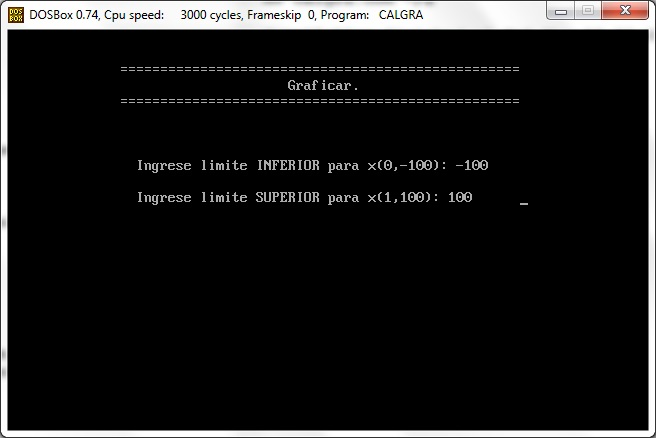
\includegraphics[scale=0.42]{img/51.jpg}

* Se grafica las funciones guardados en memoria\\

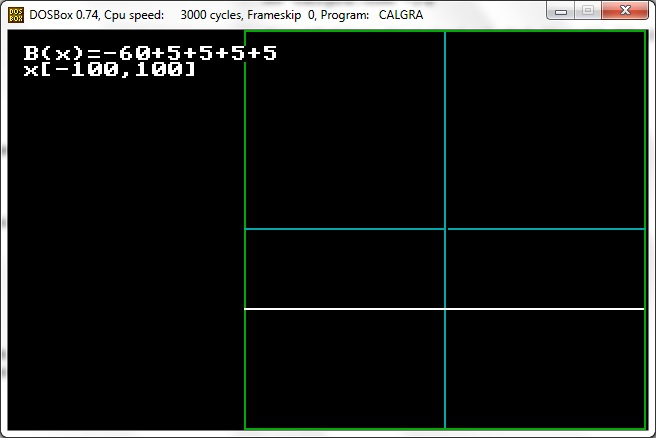
\includegraphics[scale=0.42]{img/52.jpg}

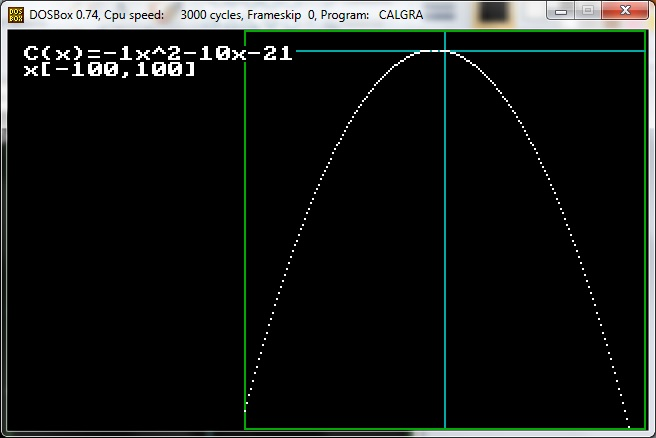
\includegraphics[scale=0.42]{img/53.jpg}

* En la esquina superir izquierda se muestra la función graficada y el
grando de graficación.\\

* Presionar cualquier tecla para regresar al menú principal\\

\section{Resolver ecuación}

* Presionar 6 en el menú principal\\

* Ingresar ecuación \\

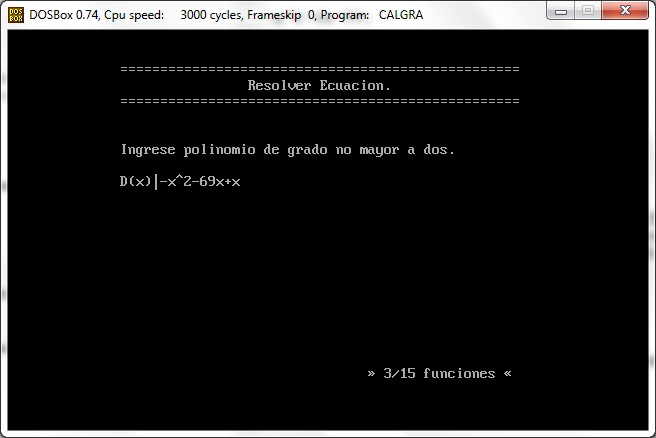
\includegraphics[scale=0.42]{img/61.jpg}

* Se muestran las soluciones o pone ''Sin solución'' si no la hay.\\

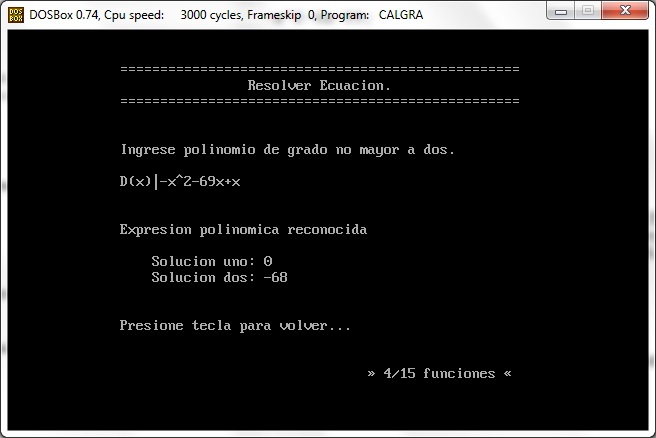
\includegraphics[scale=0.42]{img/62.jpg}

* Presionar cualquier tecla para regresar al menú principal\\


\section{Reportes}

* Presionar 7 en el menú principal\\

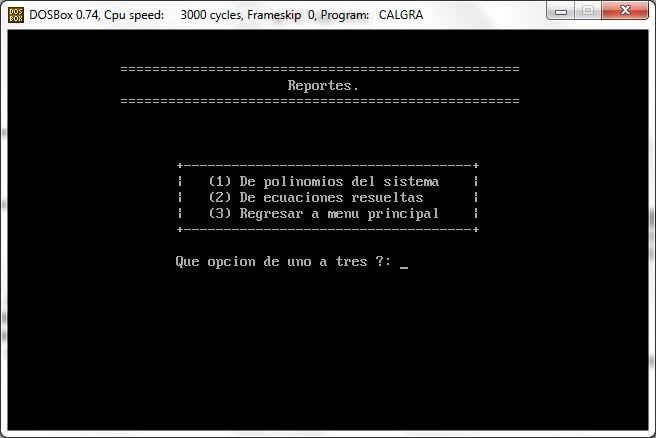
\includegraphics[scale=0.42]{img/71.jpg}

* Ingrese 1 para el reporte de polinomios del sistema. \\

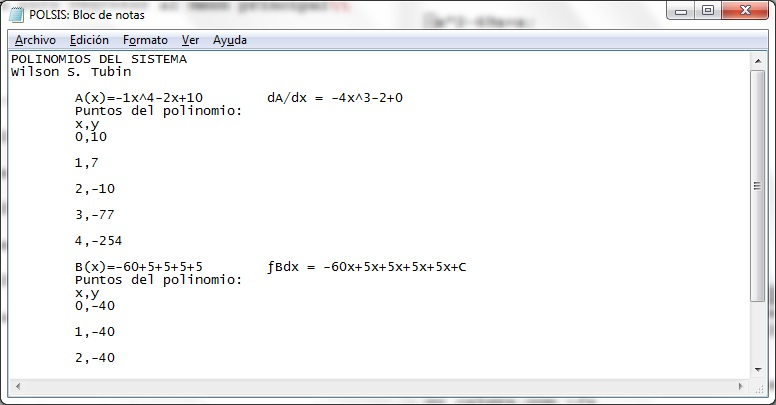
\includegraphics[scale=0.42]{img/72.jpg}

* Ingrese 2 para el reporte de ecuaciones resueltas. \\

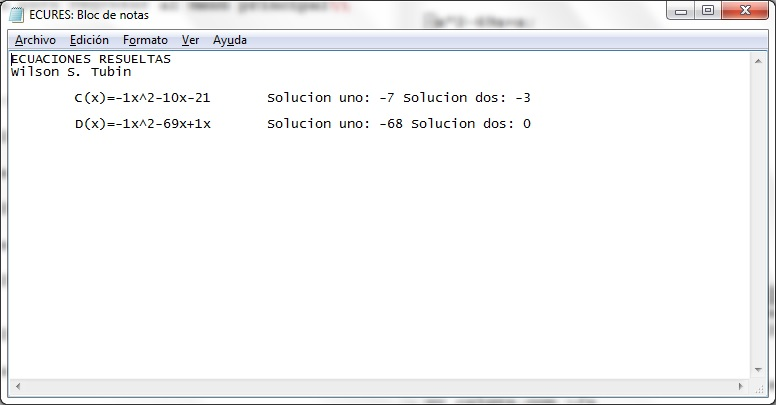
\includegraphics[scale=0.42]{img/73.jpg}


* Presione 3 para regresar al menu principal\\

\section{Salir}

* Presione 8 para terminar la ejecución del programa.


\section{Ejemplos de entrada}

\subsection{Integrar y derivar}


Ejemplos para derivar e integrar. Tomar en cuenta que solo maneja
enteros por lo que cuando se integra algo como $5x^3$ da algo como
$0x^4$. Esto es porque la división de $5$ entre $4$ no es entera.
\begin{verbatim}
+7+4x^3;

-10x+50;

-2x+1-3x^2;

-8x^3+50;

+6x^2-2x+3;

-9x^2+10+3x^2;

+3x^2-4x^3+47;

-4x^3+99+x^4-3x^2-1;

-60+5+5+5+5;

-x^4-2x+10;

+1+4x+6x^2+4x^3;

\end{verbatim}

\subsection{Integrar y derivar con errores}

Esto son ejemplos de entradas para derivar e integrar que incluyen
errores que puede identificar.

\begin{verbatim}
+7+
4x^3;

-10x^5+50;

-2 x
  + 1- 3
      x^    2;


-8x  x  ^ 3

       +50;

+6x^2-2x+3;

-9x^#2+10+x^4;

+  3x^2
        -4 x ^ 3
               +4    7  ;

4x^3+99+x^4-3x^2-1;

-60+5+5+5+5;

-10x^4-2x+109;

+1+4x+6x^2+4x^3;

-99-43-71+x^4+0;

-99-43-71+x^4+0+61;

\end{verbatim}


\subsection{Resolver}
Estas son ejemplos de entrada de ecuaciones que puede resolver.

\begin{verbatim}
-x^2-10x-21;

-x^2-69x+x;

+x^2-14x+79;

-x^2-6x-99;

+x^2+18x+81;

+x^2-49; 

-x^2+81;

-10x+50;

\end{verbatim}

\subsection{Resolver con errores}
Estos son ejemplos de entrada de ecuaciones que puede resolver que
incluyen errores que reconoce.

\begin{verbatim}
--x^2-10x-21;

+x
   ^2-
    1
4
x+7    9;

-x^2-69x+x;

-6x-"x^2-9;

+x^2+18x^6+81;

-4
   9
 +
x
   ^
2; 

+81-x^2+x^4;

-10x+50;

-10x+5&0;

-10x-x+22;

-10x-x+1+2;

\end{verbatim}


\subsection{Gráficas grado 1}

Ejemplos de funciones de grado uno que puede graficar.
\begin{verbatim}
+x;

-x;

+50x;

-10x+50;

+80+37x;

+75+0x;

-80;

-5x+3;

\end{verbatim}

\subsection{Gráficas grado 2}
Ejemplos de funciones de grado dos que puede graficar.

\begin{verbatim}
+x^2;

-x^2;

+x^2-x+3;

-x+1-3x^2;

\end{verbatim}

\subsection{Gráficas grado 3}

Ejemplos de funciones de grado tres que puede graficar.
\begin{verbatim}
+x^3;

-x^3;

+7+x^3;

-2x^3+1;

+x^3+x;

+x^3+x+4;

+x^2-x^3+47;

+x^2+x^3+5;

+1+x+x^2+x^3;

\end{verbatim}

\subsection{Gráficas grado 4}

Ejemplos de funciones de grado cuatro que puede graficar.
\begin{verbatim}
+x^4;

-x^4;

+3+1+2+x^4;

+2x^4;

-x^4-2x+10;

-7x^2+10+x^4;

-x^3+99-x^4-x^2-1;

\end{verbatim}

\section{Conclusión}
El lenguaje ensamblador es de bajo nivel y ayuda a compreder mejor el
funcionamiento de los registros y memoria de una computadora. Así
mismo DOS escribir un programa en ensamblador, para DOSBox ayuda a
tener una mejor panorámica sobre las bases de sistemas operativos mas
actuales como MS-Widonws.


% if have a single appendix:
%\appendix[Proof of the Zonklar Equations]
% or
%\appendix  % for no appendix heading
% do not use \section anymore after \appendix, only \section*
% is possibly needed

% use appendices with more than one appendix
% then use \section to start each appendix
% you must declare a \section before using any
% \subsection or using \label (\appendices by itself
% starts a section numbered zero.)
%



% \appendices
% \section{Secuencia para controlar motores paso a paso bipolares}


% use section* for acknowledgment
% \section*{Acknowledgment}


% The authors would like to thank...


% Can use something like this to put references on a page
% by themselves when using endfloat and the captionsoff option.
\ifCLASSOPTIONcaptionsoff
  \newpage
\fi

% trigger a \newpage just before the given reference
% number - used to balance the columns on the last page
% adjust value as needed - may need to be readjusted if
% the document is modified later
%\IEEEtriggeratref{8}
% The "triggered" command can be changed if desired:
%\IEEEtriggercmd{\enlargethispage{-5in}}

% references section

% can use a bibliography generated by BibTeX as a .bbl file
% BibTeX documentation can be easily obtained at:
% http://mirror.ctan.org/biblio/bibtex/contrib/doc/
% The IEEEtran BibTeX style support page is at:
% http://www.michaelshell.org/tex/ieeetran/bibtex/
%\bibliographystyle{IEEEtran}
% argument is your BibTeX string definitions and bibliography database(s)
%\bibliography{IEEEabrv,../bib/paper}
%
% <OR> manually copy in the resultant .bbl file
% set second argument of \begin to the number of references
% (used to reserve space for the reference number labels box)


% biography section
% 
% If you have an EPS/PDF photo (graphicx package needed) extra braces are
% needed around the contents of the optional argument to biography to prevent
% the LaTeX parser from getting confused when it sees the complicated
% \includegraphics command within an optional argument. (You could create
% your own custom macro containing the \includegraphics command to make things
% simpler here.)
%\begin{IEEEbiography}[{\includegraphics[width=1in,height=1.25in,clip,keepaspectratio]{mshell}}]{Michael Shell}
% or if you just want to reserve a space for a photo:

% \begin{IEEEbiography}{Michael Shell}
% Biography text here.
% \end{IEEEbiography}

% if you will not have a photo at all:
\begin{IEEEbiographynophoto}{W.~E.~S.~Tubín (201213139)}
nació en Guatemala, Guatemala. Estudia ingeniería en Ciencias y
Sistemas en la Universidad de San Carlos de Guatemala.
\end{IEEEbiographynophoto}


% insert where needed to balance the two columns on the last page with
% biographies
%\newpage

% \begin{IEEEbiographynophoto}{Jane Doe}
% Biography text here.
% \end{IEEEbiographynophoto}

% You can push biographies down or up by placing
% a \vfill before or after them. The appropriate
% use of \vfill depends on what kind of text is
% on the last page and whether or not the columns
% are being equalized.

\vfill

% Can be used to pull up biographies so that the bottom of the last one
% is flush with the other column.
%\enlargethispage{-5in}



% that's all folks
\end{document}